\documentclass[12pt]{article}
\usepackage[T1]{fontenc}
\usepackage[utf8]{inputenc} 
\usepackage[a4paper]{geometry}
\usepackage{gensymb}
\geometry{a4paper, margin=1in}
\usepackage{natbib}
\usepackage{hyperref}
\usepackage{booktabs}
\usepackage{threeparttable}
\usepackage{amssymb}
\usepackage{amsmath}
\usepackage{graphicx}
\title{Assignment 4}
\author{Dmitrii Kuptsov}
% \date{March 2025}
\begin{document}
\maketitle
\section*{Task 1}

\subsection*{Task 1.a}

\subsubsection*{Task 1.a.iii}

This confidence region shows that estimates of $x_3$ and $x_4$ are negatively correlated. From that we can conclude that (as is clear from dgp) we can recover the coefficient for $x_3 + x_4$ quite well, but the individual coefs have larger variance. It happens because $x_4$ is generated as $x_3$ + noise. This graph also shows, that we can reject the hypothesis $x_3 = x_4 = 0$. In comparison, we couldn't reject the hypothesis that $x_3 = 0$ or $x_4 = 0$ separately.

\subsubsection*{Task 1.a.iv}

When we test significance of the regressors separately in this case we cannot reject the null, because 0 is in the confidence interval. However, when we test jointly, (0, 0) is quite far from the confidence ellipsis, which means that both regressors can hardly be insignificant at the same time.

It is especially relevant for the collinear regressors, because when the regressors have little collinearity, joined test would be somewhat similar to the separate ones. However, if the regressors are highly collinear, like in this case, it would be hard for the model to distinguish between these regressors. It would lead to high CIs. In comparison, joined test will be much more helpful, because the coef for the sum of these regressors would have smaller CIs (if there are no other strong collinearities in the model).

\subsection*{Task 1.b}

\subsubsection*{Task 1.b.i}

Estimates became much more precise for all of the coefs. (Reason: increase in the number of observation leads to the decrease of the variance.) However, for $x_2$ the variance is again considerably smaller than for $x_3$ and $x_4$. Therefore, collinearity problem decreased due to the larger sample, but haven't been totally solved.

\subsubsection*{Task 1.b.ii}

CIs became much smaller, all of them contain the true values. Again, this happens because of the decrease in variance. We can see that CI for $x_2$ is few times smaller than CIs for $x_3$ and $x_4$, with the same true coefficients. This is the effect of collinearity.

\subsubsection*{Task 1.b.iii}

The confidence region has the same form as in the previous step. It is still an ellipsis due to the collinearity, but it has decreased considerably. It is still very close to the line $x_3+x_4=1$, because the coefficients for sum of the regressors have much lower variance than the coefs itself again due to the collinearity.

\subsubsection*{Task 1.b.iv}

$var(\hat\beta|X) = \sigma \cdot (XX^T)^{-1}$, so $var(\hat\beta_3|X) = \sigma \cdot (\sum_i x_{i3} \cdot x_{i3})^{-1}$. Therefore, $var(\hat\beta_3|X)$ decreases proportionally to $\frac{1}{n}$ with the number of observations. As a result, standard deviation decreases and confidence intervals became smaller.

\subsection*{Task 1.c}

\subsubsection*{Task 1.c.i}

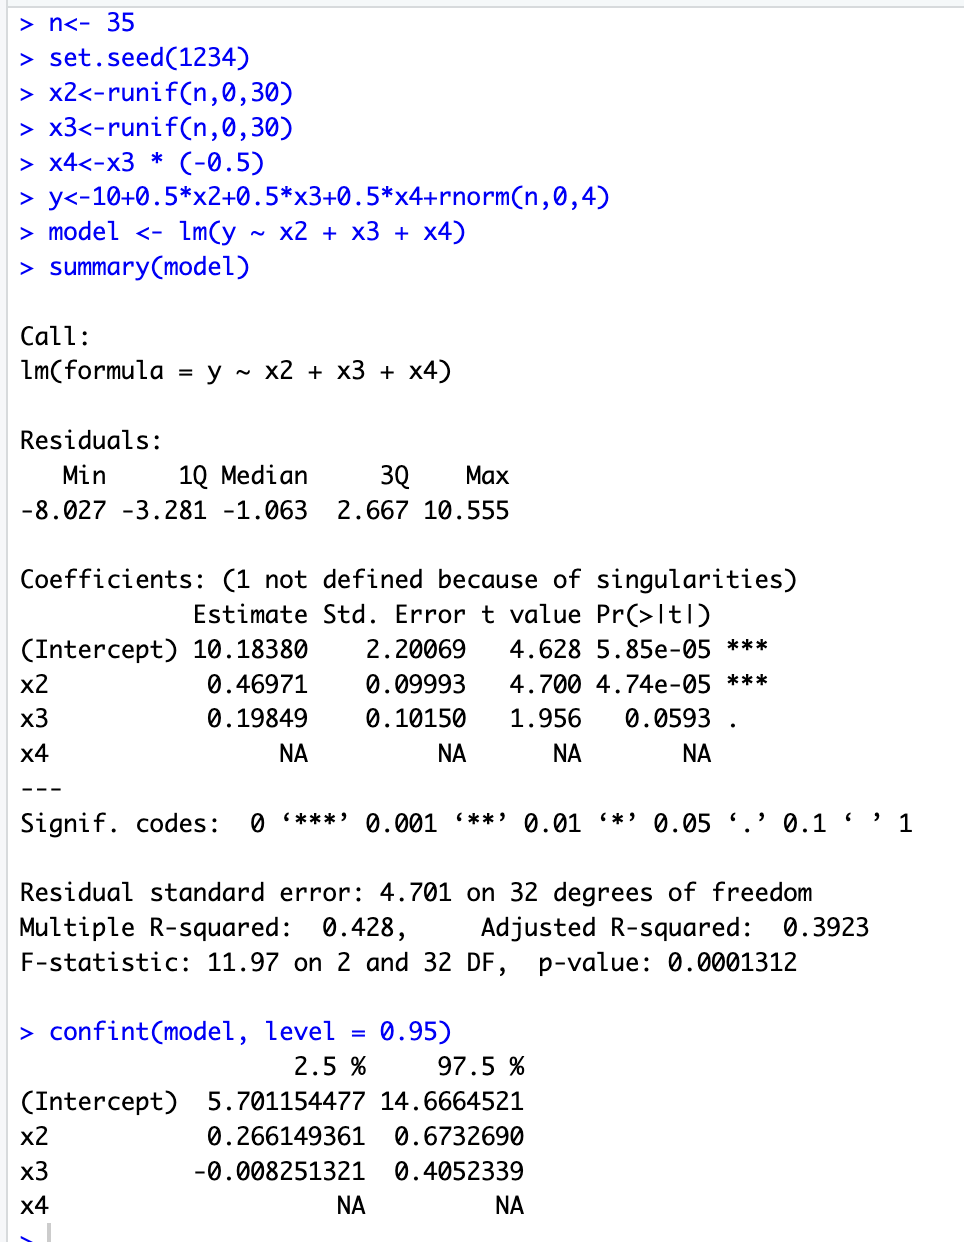
\includegraphics[width=0.8\textwidth]{1_c_i.png}

\subsubsection*{Task 1.c.ii}

We got an estimate only for $x_3$, $x_4$ was excluded due to the perfect collinearity. We can substitute $x_4$ with $-0.5\cdot x_3$, and the true coefficient of $x_3$ with excluded $x_4$ would be 0.25 ($\beta_3 \cdot x_3 + \beta_4 \cdot x_4 = x_3 \cdot (\beta_3 - 0.5\beta_4)$). Therefore, we got one estimate for $(\beta_3 - 0.5\beta_4)$, and infinite number of estimates for each particular parameter. 


\end{document}
